\section{3D Printed Parts}
Here is a list of 3D-printed parts I printed or plan to print:

\begin{figure}[h]
    \centering
    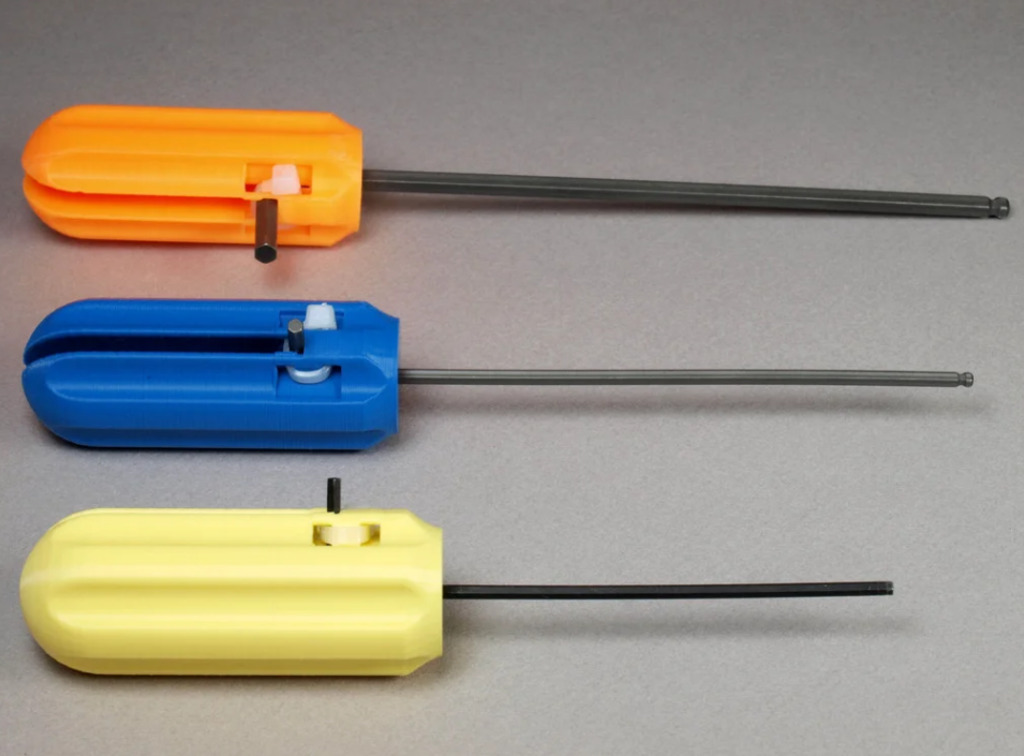
\includegraphics[width=\textwidth,height=5cm,keepaspectratio=true]{3DHandle}
    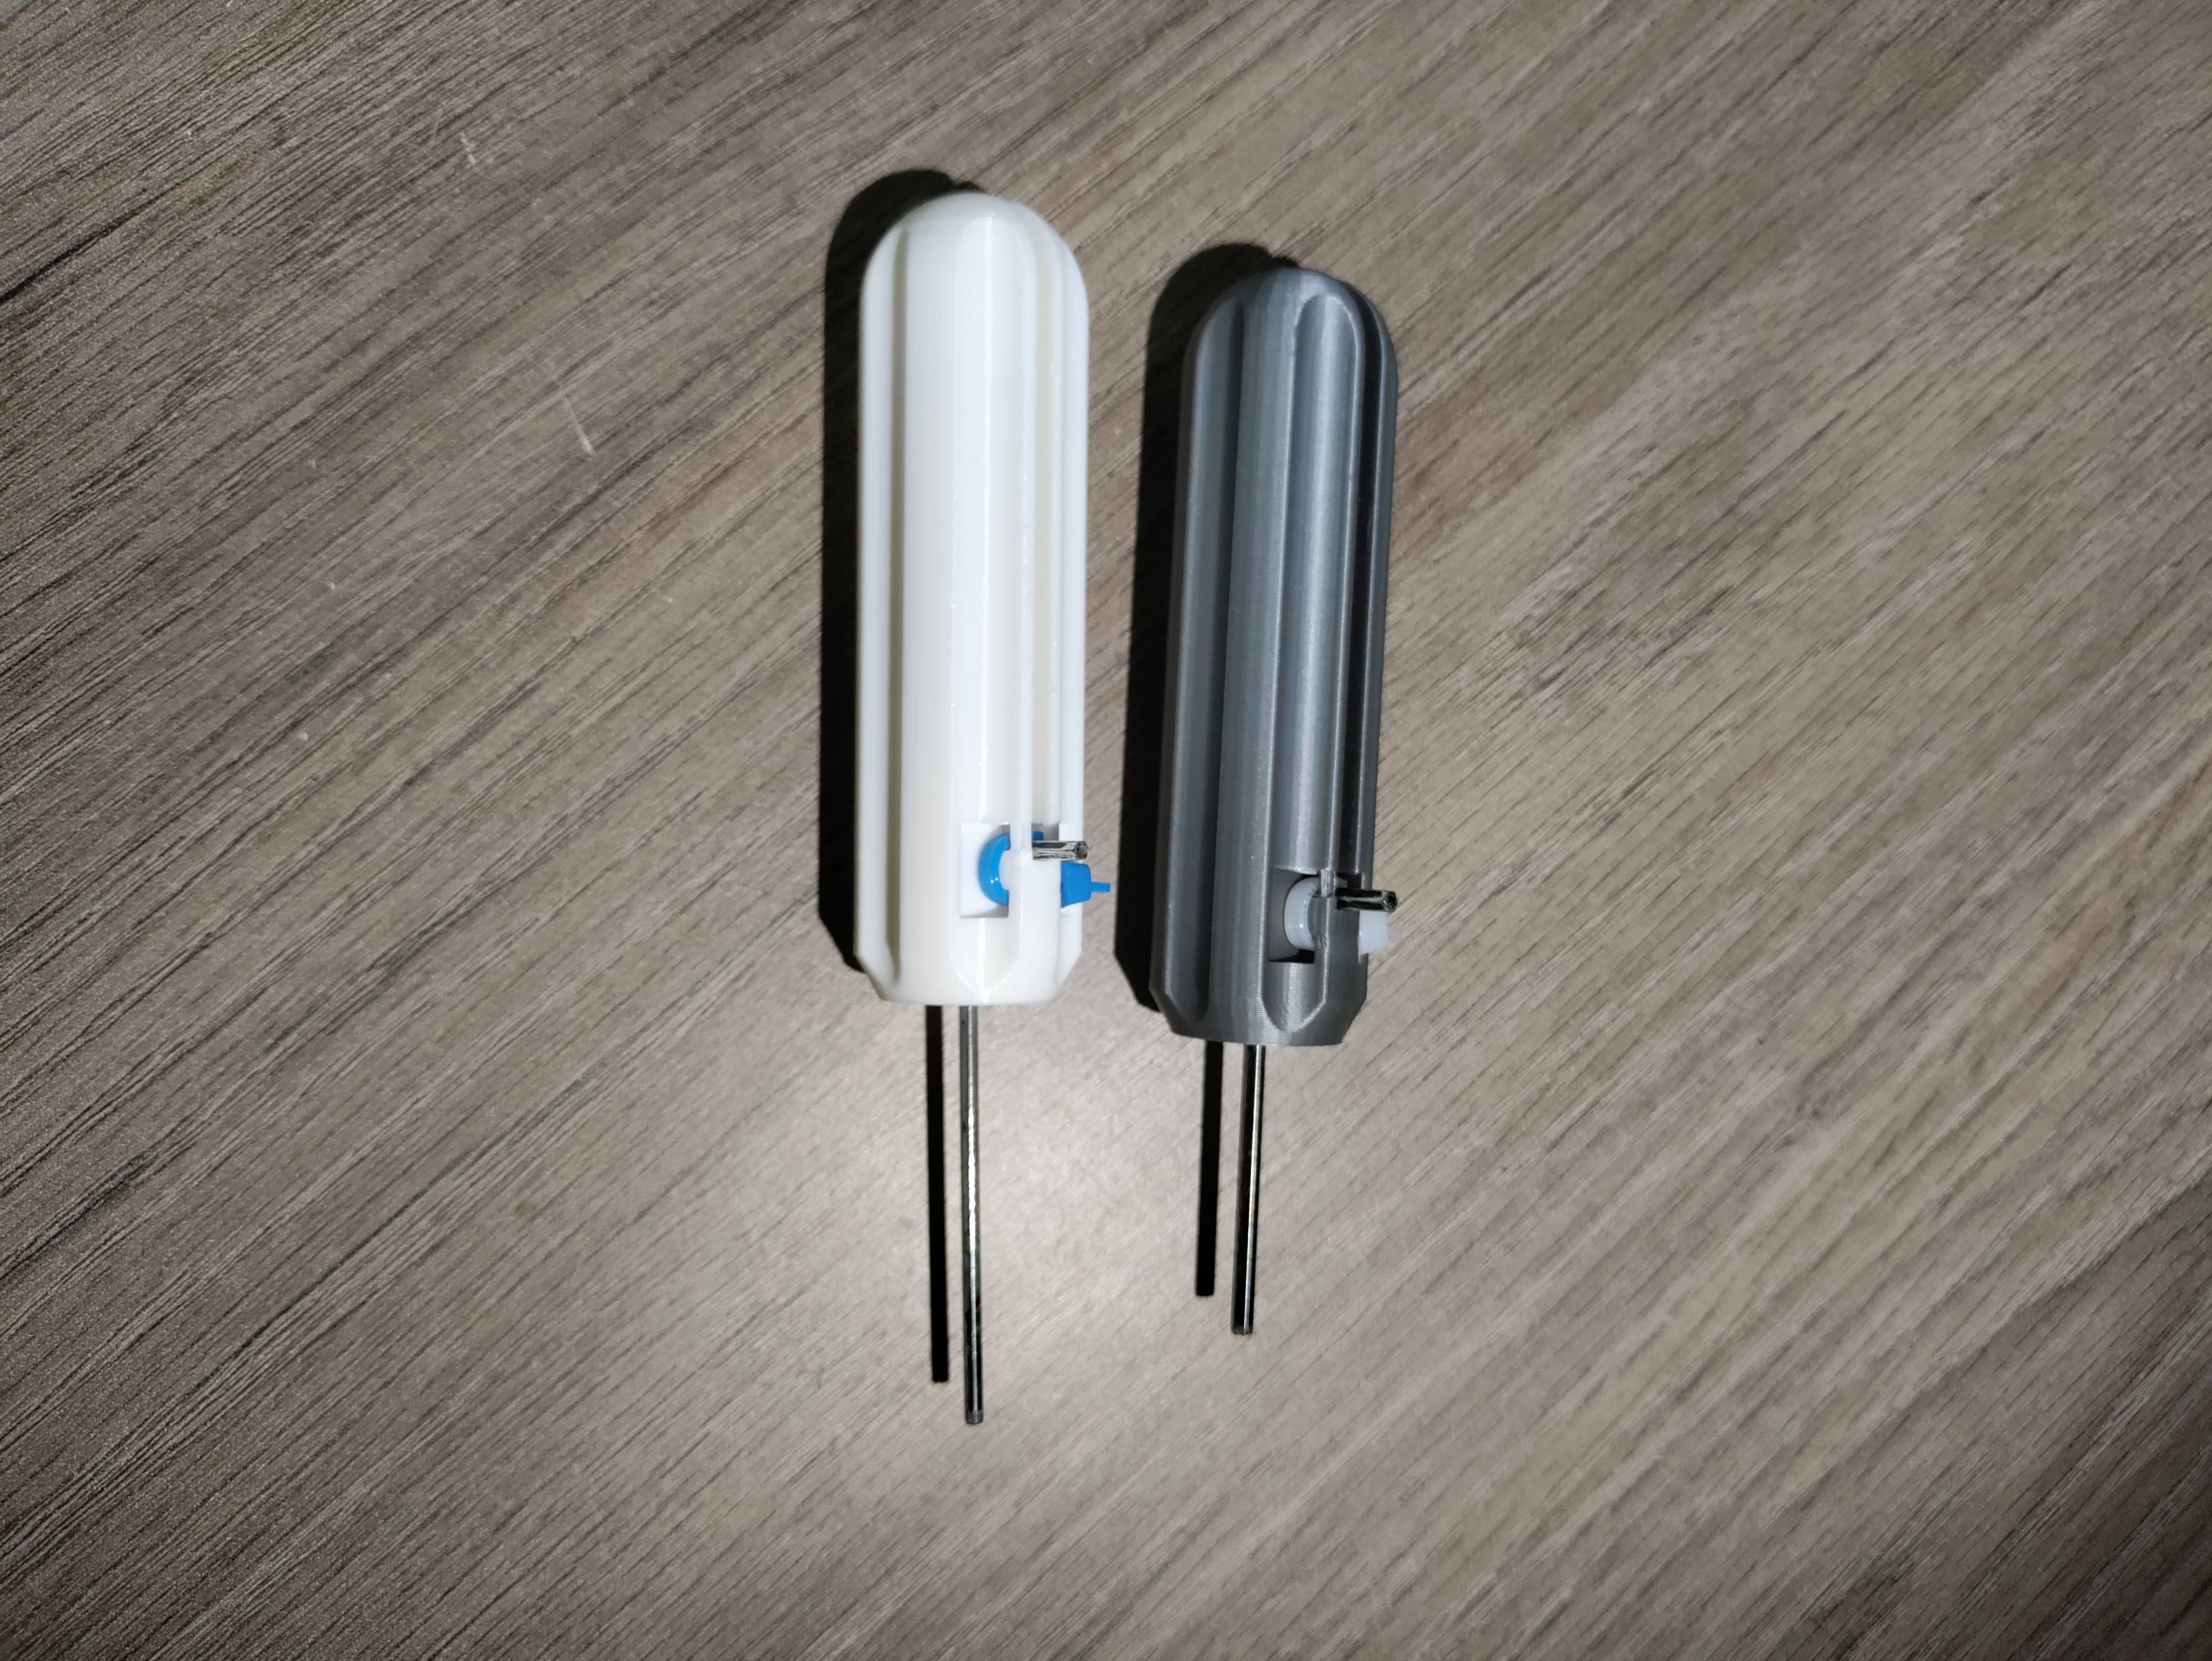
\includegraphics[width=\textwidth,height=5cm,keepaspectratio=true]{3DHandleCustom}
    \caption{
        A handle for hex wrenches held together by a zip tie; It's very quick to use, provides slightly more torque, and is a lot easier to hold. (Left) The original. \cite{3DHandle} (Right) My modification; I made the handle longer.
    }
\end{figure}


\begin{figure}[h]
    \centering
    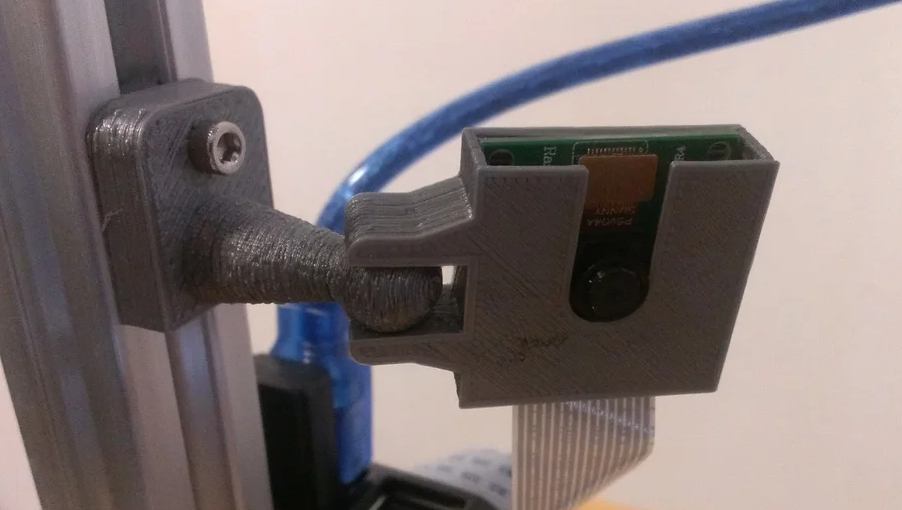
\includegraphics[width=\textwidth,height=5cm,keepaspectratio=true]{3DRasp}
    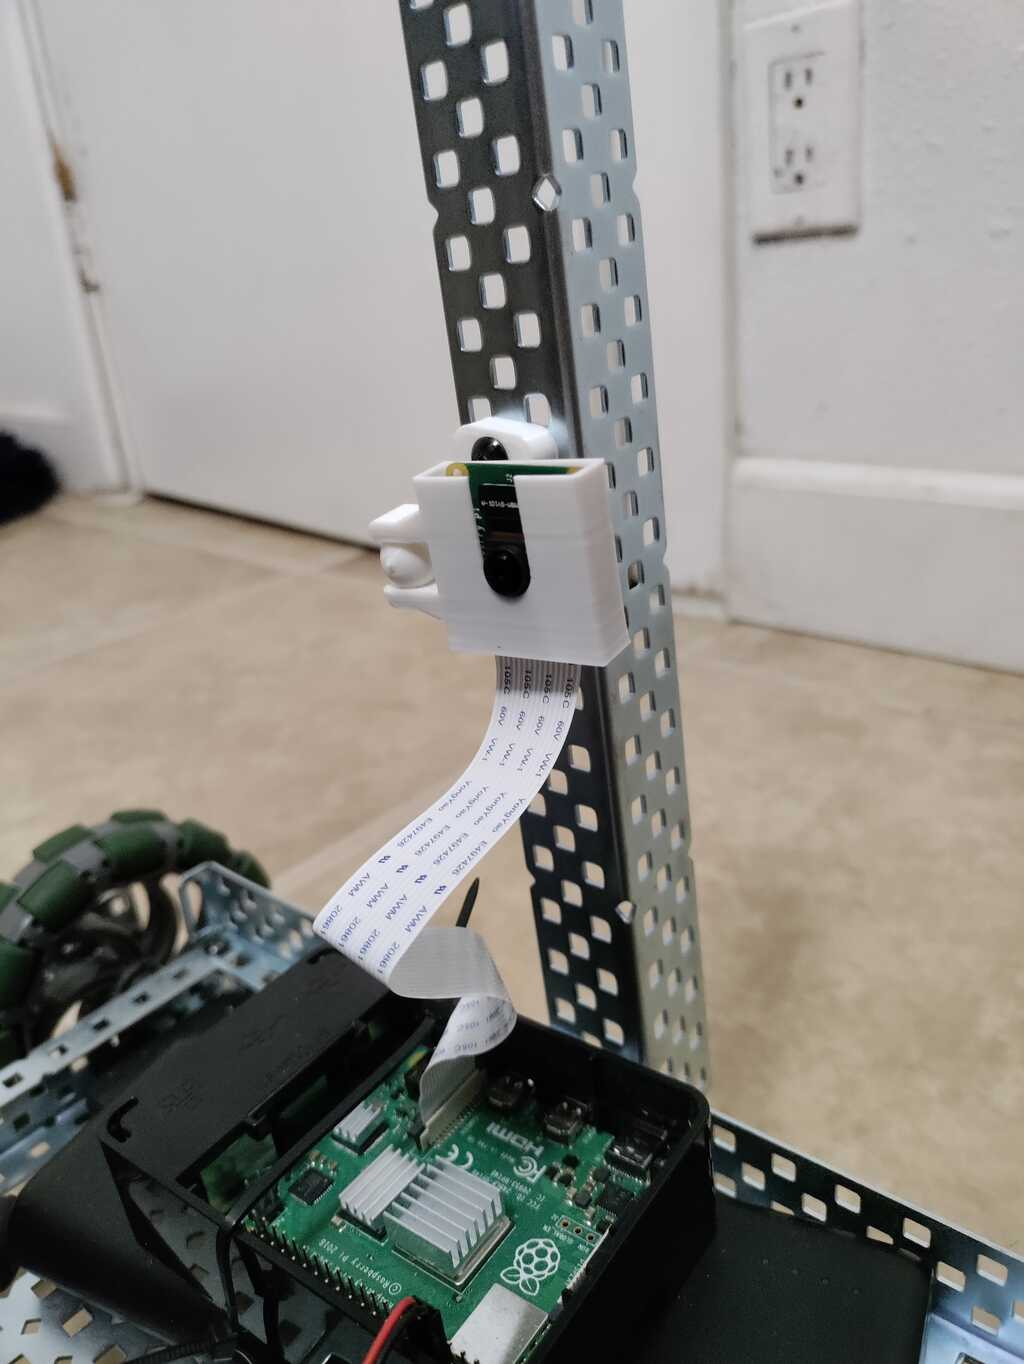
\includegraphics[width=\textwidth,height=5cm,keepaspectratio=true]{3DRaspCustom}
    \caption{
        A stand meant to hold the camera for a Raspberry Pi. (Left) The original. \cite{3DRasp} (Right) My modification; Made the hole big enough to fit VEX screws.
    }
\end{figure}

\begin{figure}[h]
    \centering
    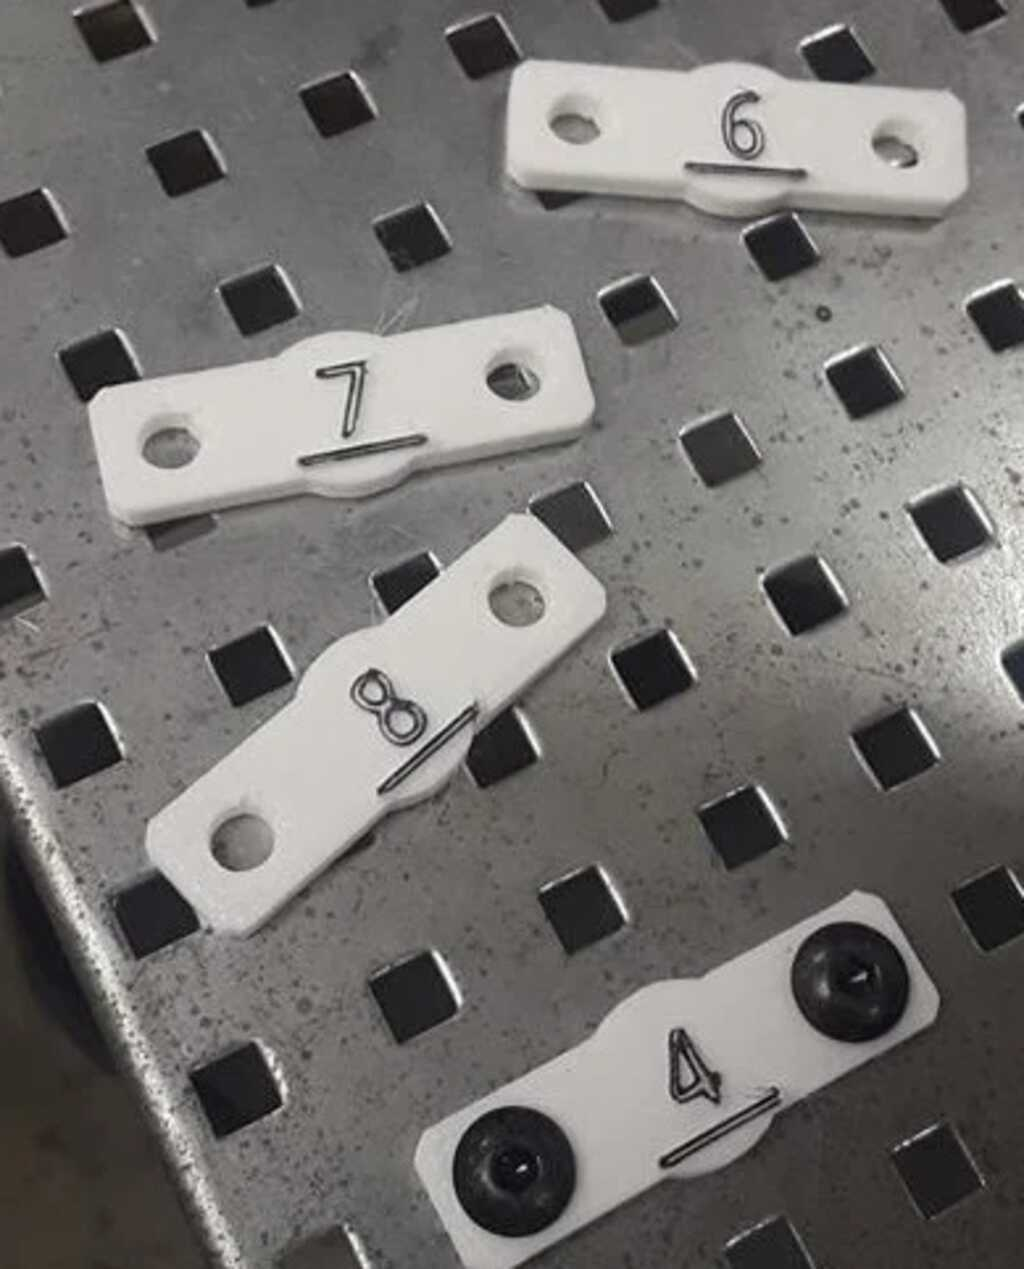
\includegraphics[width=\textwidth,height=5cm,keepaspectratio=true]{3DTag}
    \caption{
        A simple numbered tag for VEX robots \cite{3DTag}; I feel like this would make it easier to remember what order our robots were built in and fight off the space-time distortion of human memory. We can make ordered map of them in a book or something with pictures for memories. It can also be a good first print for our Ultimaker S3.
    }
\end{figure}
